\documentclass[11pt]{article}

% ---------- Preamble ----------
\usepackage[margin=1in]{geometry}
\usepackage{amsmath,amssymb,amsthm,mathtools}
\usepackage{booktabs}
\usepackage{multirow}
\usepackage{makecell}
\usepackage{graphicx}
\usepackage{xcolor}
\usepackage{enumitem}
\usepackage{microtype}
\usepackage[font=small,labelfont=bf,skip=6pt]{caption}
\usepackage[colorlinks=true,linkcolor=blue!60!black,citecolor=blue!60!black,urlcolor=blue!60!black]{hyperref}
\usepackage[capitalize,noabbrev]{cleveref}

\newtheorem{definition}{Definition}
\emergencystretch=1.5em

% Placeholder figure box
\newcommand{\figplaceholder}[1]{%
  \fbox{\parbox{0.94\linewidth}{\centering\vspace{2.2em}\textsc{Figure placeholder}\vspace{0.4em}\\ \small #1 \vspace{2.2em}}}}

% Visible TODO placeholder (never guess a missing fact)
\newcommand{\todo}[1]{\textcolor{red}{\textbf{[TODO: #1]}}}

% Estimand macros
\newcommand{\accfc}{\mathrm{Acc}_{\mathrm{FC}}}
\newcommand{\accfree}[1]{\mathrm{Acc}_{\mathrm{free}}(#1)}
\newcommand{\accro}[1]{\mathrm{Acc}_{\mathrm{ro}}(#1)}
\newcommand{\accrev}[1]{\mathrm{Acc}_{\mathrm{rev}}(#1)}
\newcommand{\dtot}[1]{\Delta_{\mathrm{tot}}(#1)}
\newcommand{\dro}[1]{\Delta_{\mathrm{ro}}(#1)}
\newcommand{\res}[1]{\rho(#1)}
\newcommand{\TV}{\mathrm{TV}}
\newcommand{\ADD}{\mathrm{ADD}}

\title{\bf Near-Lossless Under Readout, Collapse Under Free Generation:\\
A Trajectory Audit of KV-Cache Compression for Reasoning}
% NOTE: this is the NAMED working/arXiv version. ICLR submission is double-blind:
% venue conversion must restore "Anonymous Authors" and re-anonymize the repo URL.
\author{Muhammad Ali Shah\\
Lahore University of Management Sciences (LUMS)\\
\texttt{27100172@lums.edu.pk}\\[3pt]
\small Working draft --- all numbers final unless marked \emph{in progress}}
\date{}

\begin{document}
\maketitle

% =====================================================================
\begin{abstract}
KV-cache eviction methods are certified near-lossless almost entirely on evidence that holds the generated text fixed --- perplexity on reference traces, few-shot accuracy, retrieval --- while the HOTT benchmark, \emph{free-running} the same eviction families on reasoning tasks, reports severe, method-specific degradation. We show both literatures are measuring correctly, on different channels of the same loss. On MATH-500 with DeepSeek-R1-Distill-Qwen-7B at cache budget 256, random eviction scores $0.765$ when the full-cache reasoning trace is teacher-forced and only the answer is generated under compression, but $0.422$ when the model writes its own trace (full cache $0.882$; StreamingLLM $0.584$ versus $0.237$; an attention-score heavy-hitter press $0.597$ versus $0.247$). The gap --- a trajectory residual of $-0.343$ / $-0.347$ / $-0.349$ across three mechanistically unrelated eviction policies, with a certified port of the reasoning-specific R-KV policy showing the same readout-invisible structure at $-0.278$ while free-running best --- is invisible to accuracy evaluation on held-fixed traces. We formalize this with an accuracy-scale decomposition of free-running loss into an on-reference readout component and a trajectory residual, and bound the residual's off-policy bias with a reverse-replay bracket that excludes zero for every policy, under problem-clustered confidence intervals on every endpoint and under every treatment of ambiguous rows. Onset-aligned per-step total-variation profiles supply the mechanism: divergence is exactly zero before the first eviction, ${\approx}0.002$ per step immediately after, and compounds roughly $50\times$ over the trajectory --- even with the trace held fixed --- so short-horizon evaluation structurally measures the pre-compounding regime. A distribution-level instrument with a two-full-cache negative control (noise floor $\approx 0.07$ versus $0.46$--$0.75$ in compression cells) shows the answer distribution is silently rewritten, overwhelmingly toward lost correct answers. We package these estimands as the \emph{trajectory audit} --- a four-step, intervention-agnostic protocol (forward readout, free-run, reverse readout, divergence profiling) for pricing what held-trace evaluation misses --- and release it as a pinned, bitwise-replayable harness. The implication is one sentence: report free-running reasoning accuracy, because readout-style metrics can certify near-losslessness while deployed accuracy has collapsed.
\end{abstract}

% =====================================================================
\section{Introduction}
\label{sec:intro}

KV-cache compression is the standard lever for serving long-context transformer inference within memory budgets: eviction policies such as StreamingLLM~\cite{xiao2023streamingllm}, H2O~\cite{zhang2023h2o}, SnapKV~\cite{li2024snapkv}, and R-KV~\cite{rkv2025} discard cached key--value entries and report that downstream quality is largely preserved --- frequently described as near-lossless --- even at aggressive compression ratios. Against this stands the HOTT benchmark~\cite{hott2025}, which evaluates the same eviction families \emph{free-running} on reasoning tasks and reports strongly \emph{method-specific} degradation, not uniform collapse: on MATH-500 with DeepSeek-R1-Distill-Qwen-7B (budgets 128--512), full-cache accuracy is $0.47$, and at budget 128 StreamingLLM falls to $0.03$ while heavy-hitter methods degrade far less (\cref{sec:related} gives the full audit). The sharpest case is StreamingLLM: certified near-lossless on its own perplexity evaluation, yet at $0.03$ free-running on MATH-500 reasoning. That single method \emph{is} the readout-vs-trajectory gap in the wild. Both literatures are internally careful; the contradiction is between what their protocols measure. This paper contributes an evaluation protocol --- the \emph{trajectory audit} --- and the measurement study it enables, which explains \emph{why} the two literatures disagree; we propose no new compression technique.

Our diagnosis begins with an observation about evaluation protocol. Most method papers evaluate in ways that hold the generated trace fixed or nearly fixed: perplexity on reference text, teacher-forced likelihoods, short-answer completions, or retrieval-style probes (R-KV, which evaluates free-running and claims gains, is the exception; \cref{sec:related} audits this and our cells test it directly, \cref{sec:threats}). All of these interrogate what we call the \emph{readout} channel: given a (good) context, can the compressed model still read the answer out of it? Free-running benchmarks such as HOTT instead let the compressed model generate its own multi-hundred-token reasoning trajectory, so any distortion the compression induces in the trajectory itself is allowed to accumulate and feed back. If compression damage were purely a readout phenomenon, the two protocols would agree. They do not, which raises the central question of this paper: \textbf{how much of the free-running accuracy loss under KV compression is attributable to readout, and how much lives in the generated trajectory itself --- and can the trajectory part be seen at all by held-fixed-trace evaluation?}

We answer with an explicit decomposition. For each compression method $m$ we measure the \emph{total} accuracy change of compressed free-running generation against a pinned full-cache reference bank; the \emph{on-reference readout} change, obtained by teacher-forcing the exact full-cache reasoning token IDs to the reasoning/answer boundary and then generating only the answer span under compression; and the \emph{residual}, defined --- and only defined --- as the accuracy change unexplained by on-reference readout. Because the readout intervention conditions on the full-cache trajectory, it is off-policy with respect to the states the compressed model actually visits, and the residual is biased toward the trajectory share~\cite{ross2011dagger}. We therefore state this caveat up front, not in rebuttal, and bound the bias symmetrically with \emph{reverse replay}: the compressed free-run trace read out under the full cache. Forward and reverse readout together bracket the on-policy residual. Two further instruments complete the suite: \emph{ADD}, a total-variation measure of answer-distribution distortion with a permutation null, a termination-versus-within-answered decomposition, and a signed flip-mass that separates gained from lost correct answers; and an onset-aligned per-step total-variation profile over teacher-forced replay, which localizes \emph{when} divergence arises relative to the first eviction event. Together, these instruments constitute the \emph{trajectory audit} (\cref{fig:protocol}), stated as a reusable, intervention-agnostic protocol in \cref{sec:conclusion}.

\paragraph{Thesis.} At aggressive cache budgets, compression damage to reasoning is real, large, and largely \emph{invisible to teacher-forced / readout-style evaluation} --- which is why method papers that evaluate on held-fixed traces report near-lossless while free-running evaluation reports severe, method-specific degradation (for StreamingLLM, collapse). The gap is the trajectory residual, and it arises from a divergence that is approximately zero at the moment of eviction and \emph{compounds} over the generated trajectory.

We emphasize what the thesis is not. We observed no accuracy \emph{gains} under compression on small-budget MATH-500, so no ``denoising'' or $>$100\%-of-baseline regime is claimed; the paper is framed strictly as near-lossless-under-readout versus collapse-under-free-generation. And throughout, divergence quantities (ADD, per-step TV, the residual) are reported as \emph{behavioral-fidelity loss}, never as ``damage to reasoning ability'': correctness is the only quality arbiter, and every divergence quantity is accompanied by its signed flip-mass.

\paragraph{Contributions.}
\begin{itemize}[leftmargin=1.6em,itemsep=2pt]
  \item \textbf{The trajectory audit}: a four-step, intervention-agnostic evaluation protocol --- forward readout, free-run, reverse readout, onset-aligned divergence profiling --- that prices what held-trace evaluation misses, with its own validity controls (negative control, self-control, resampling calibration, exact replication), released as a pinned, bitwise-replayable harness (\cref{sec:estimands,sec:conclusion}).
  \item \textbf{A resolution of the near-lossless-under-readout versus degraded-under-free-running contradiction} via an accuracy-scale decomposition of compressed free-running loss into on-reference readout and a trajectory residual, with the residual explicitly framed as a definition (``accuracy change unexplained by on-reference readout''), not a measured cause (\cref{sec:estimands}).
  \item \textbf{The powered phenomenon}: at budget 256 on MATH-500 (DeepSeek-R1-Distill-Qwen-7B), full-cache accuracy $0.882$ collapses to $0.237$ (StreamingLLM) and $0.422$ (Random); random eviction beats the principled recency policy by $+0.185$, 95\% CI $[0.130, 0.242]$, with per-problem difference $\ge 0$ on 94/100 problems (44 strict wins, 50 ties, 6 losses) --- an architecture-dependent ordering: it reverses on the Llama base (\cref{sec:phenomenon,sec:threats}).
  \item \textbf{A large, readout-invisible trajectory residual} of $\approx -0.34$ across three mechanistically unrelated eviction policies (uniform, positional, attention-score; residual spread $0.006$, every CI excluding zero; 400 conditions per cell), with the method differences living in the readout channel --- on the forward estimand, a residual of similar magnitude exists for every policy tested, reported as exploratory (\cref{sec:forward}).
  \item \textbf{An off-policy defense}: forward and reverse readout give two $\text{total}-\text{readout}$ residual estimates whose min/max bracket excludes zero for every policy (Random $[-0.343,-0.246]$, StreamingLLM $[-0.466,-0.347]$, H2O-style $[-0.463,-0.349]$, R-KV $[-0.278,-0.221]$), with problem-clustered 95\% CIs on all eight endpoints excluding zero --- so the central claim survives the covariate-shift correction with statistical significance, while the \emph{method-level} readout-vs-trajectory attribution is reported as estimand-dependent and exploratory (\cref{sec:reverse}).
  \item \textbf{The mechanism}: onset-aligned TV profiles over 800 replays show divergence of exactly $0.0000$ before the first eviction, $0.0018$ in the first 50 post-eviction steps, compounding to $0.0884$ later --- slow-compounding drift that single-step evaluation structurally misses (\cref{sec:mechanism}).
  \item \textbf{Instrument validity}: a two-full-cache negative control establishing an ADD noise floor of $\approx 0.07$ (mean permutation $p = 0.976$, 0\% of problems significant) against compression-cell ADD of $0.46$--$0.75$, plus a Jaccard-1.0 retained-set parity certification of our R-KV port (\cref{sec:control}).
\end{itemize}

\paragraph{Summary of findings.} At budget 256 every eviction policy tested loses most of its free-running accuracy, but teacher-forced readout recovers much of it: readout accuracy is $0.765$ (Random), $0.584$ (StreamingLLM), and $0.597$ (H2O-style) against free-running $0.422$, $0.237$, and $0.247$ --- trajectory residuals of $-0.343$, $-0.347$, and $-0.349$. Reverse replay confirms the residual is not an off-policy artifact: reading the compressed trajectory out under a \emph{full} cache recovers only to $0.636$ and $0.417$, far below the $0.882$ reference. The certified R-KV port --- the best free-runner at $0.520$ --- shows the same structure: readout $0.798$, residual $-0.278$, bracket excluding zero. The per-step TV profile places the origin of this loss after the first eviction with near-zero immediate effect and strong compounding, and ADD shows the two methods distort the answer distribution through different channels --- StreamingLLM almost entirely within-answered (it keeps answering, but wrongly; ADD $0.751$, signed flip-mass $-0.646$), Random with a larger termination-mass shift ($+0.224$; it rambles and fails to terminate). Our pre-registered read of the powered decomposition came out \textsc{complicate}: the central residual is robust, but the pilot's clean ``StreamingLLM$=$readout / Random$=$trajectory'' double dissociation did not survive powering.

% =====================================================================
\section{Related Work}
\label{sec:related}

\subsection{KV-cache eviction methods and how they evaluate}
StreamingLLM~\cite{xiao2023streamingllm} retains attention sinks plus a recent window; H2O~\cite{zhang2023h2o} retains heavy-hitter tokens by accumulated attention mass; SnapKV~\cite{li2024snapkv} selects entries by observation-window attention prior to generation; R-KV~\cite{rkv2025} targets redundancy in reasoning traces specifically. Eviction is one of several compression families --- quantization (e.g., KIVI~\cite{liu2024kivi}) and merging store all entries at reduced fidelity rather than discarding them --- and we scope this study to decoding-time eviction, the family HOTT evaluates and the one whose near-lossless certifications conflict with free-running results. The crux for this paper is not the eviction policies but their \emph{evaluation protocols}, audited in \cref{tab:audit}. For three of the four, the primary near-lossless evidence is readout-shaped: StreamingLLM's is language-modeling perplexity on held reference text (PG19, streaming to 4M tokens); H2O's is few-shot task accuracy under lm-eval plus summarization (XSUM/CNN) and throughput; SnapKV's is LongBench and needle-in-a-haystack retrieval. Each of these either holds the trace fixed or keeps generations short enough that trajectory feedback cannot accumulate; in our terminology (\cref{sec:estimands}), they estimate the readout channel. \textbf{R-KV is the counterexample, not an instance}: it evaluates MATH-500 and AIME-24 \emph{free-running} and claims $105\%$ of full-KV accuracy at ${\sim}16\%$ cache (R1-Distill-Llama-8B, AIME-24) --- a claimed $>$100\% regime that our R-KV cells test directly rather than explain away (no such regime at 7B: on small-budget MATH-500 our certified port free-runs at $0.520$ against the $0.882$ reference, \cref{sec:forward}, and on AIME-24 at budget 2048 the best press reaches $0.283$ versus the $0.371$ reference, \cref{sec:threats}). For the readout-evaluated majority, none of the primary evidence estimates the accuracy of a long, free-running, compression-active reasoning trajectory --- the quantity a deployed reasoning model actually delivers. This is the evaluation gap through which a $\approx -0.34$ trajectory residual can pass unobserved.

\begin{table}[t]\centering
\caption{Evaluation-protocol audit. Near-lossless claims for eviction methods rest on
readout-shaped evidence; only R-KV reports free-running reasoning accuracy (and claims gains
--- the regime our cells test directly, \cref{sec:threats}, not one we explain away).}\label{tab:audit}\footnotesize
\setlength{\tabcolsep}{4pt}
\begin{tabular}{llp{5.6cm}cc}
\toprule
Method & Venue & Primary near-lossless evidence & Trace fixed? & \makecell{Free-run\\ reasoning acc?} \\
\midrule
StreamingLLM & ICLR'24 & LM perplexity (PG19, streaming to $4$M tok) & Yes & No \\
H2O & NeurIPS'23 & few-shot task acc.\ (lm-eval), summ.\ (XSUM/CNN), throughput & Mostly & No \\
SnapKV & NeurIPS'24 & LongBench, Needle-in-a-Haystack retrieval & Yes & No \\
R-KV & NeurIPS'25 & \textbf{MATH-500, AIME-24 free-running}; $105\%$ full-KV @ ${\sim}16\%$ cache & No & \textbf{Yes} \\
\bottomrule
\end{tabular}\end{table}

\subsection{Reasoning under compression}
The HOTT benchmark (\emph{Hold Onto That Thought})~\cite{hott2025} evaluates the same eviction families free-running on reasoning tasks, with strongly method-dependent outcomes rather than uniform collapse: at budget 128 on R1-Distill-Qwen-7B MATH-500 (HOTT Table 2, budgets 128/256/384/512), StreamingLLM falls to $0.03$ against a full-cache baseline of $0.47$, while H2O ($0.14$) and SnapKV ($0.38$) degrade far less; HOTT's verbatim conclusion is that \emph{``heavy-hitter methods H2O and SnapKV-D win over all budgets and datasets for reasoning models''}. Set against the method papers' own near-lossless certifications (\cref{tab:audit}), this is the contradiction we decompose --- sharpest for StreamingLLM, near-lossless under its own perplexity protocol and at $0.03$ under HOTT's free-running one. We do not merge HOTT's numbers with ours digit-for-digit: the baselines differ (HOTT's full-cache MATH-500 accuracy is $0.47$ versus our $0.882$, reflecting different decode-length and sampling configurations; our $0.882$ is in line with the $0.928$ MATH-500 pass@1 reported for this model at full decode length~\cite{deepseek2025r1}). What we reconcile is the \emph{channel structure}: method-paper near-losslessness lives in the readout channel, HOTT's free-running degradation lives in the trajectory channel, and the residual is their difference --- both sets of numbers can be simultaneously correct because they measure different channels of the same underlying loss. We use the same library stack HOTT used (kvpress) for comparability, including its H2O-style \texttt{ObservedAttentionPress} labeling (\cref{sec:setup}). Three further critical strands corroborate the evaluation gap without explaining it: degradation under compression is highly non-uniform across instruction types, so averaged accuracy hides failure structure~\cite{pitfalls2025}; worst-case lower bounds limit lossless cache compressibility~\cite{barriers2025}; and synthetic-probe analyses trace long-\emph{input} compression damage to structural attention-routing effects~\cite{physics2026}. None of these lines separates readout from trajectory on an accuracy scale, which is the decomposition this paper contributes.

\subsection{Teacher forcing versus free running}
That teacher-forced evaluation can diverge sharply from free-running behavior is a classical observation: exposure bias in sequence models~\cite{ranzato2016exposure,bengio2015scheduled} and the covariate-shift analysis of imitation learning~\cite{ross2011dagger} both formalize how errors compound when a model consumes its own outputs, with regret growing superlinearly in horizon under distribution shift. Our forward readout estimand is deliberately off-policy in exactly the DAgger sense --- it conditions on reference states --- and we import that lineage's discipline: the residual is stated as biased toward the trajectory share, and the bias is bounded empirically (reverse replay) rather than argued away. We retain total variation over KL/JSD for per-step divergence because $1 - \text{acceptance} \approx \TV$ in speculative decoding~\cite{leviathan2023speculative}, giving TV a direct behavioral reading; JSD is an appendix sensitivity. To our knowledge, no prior work applies this teacher-forcing-versus-free-running lens \emph{quantitatively, on an accuracy scale}, to KV-cache compression of reasoning models, which is the specific measurement this paper contributes.

% =====================================================================
\section{Estimands and Experimental Design}
\label{sec:estimands}

\subsection{Setup}
\label{sec:setup}
\textbf{Model and benchmark.} DeepSeek-R1-Distill-Qwen-7B~\cite{deepseek2025r1} on MATH-500~\cite{hendrycks2021math,lightman2023verify}, sampled at temperature $0.6$, top-$p$ $0.95$, seeds frozen in configuration.

\textbf{Full-cache reference.} A single pinned canonical full-cache (FC) bank: 250 problems $\times$ $n{=}8$ seeds $=$ 2000 generations, FC accuracy $\accfc = 0.882$. Every accuracy change in this paper is computed against this one bank by construction.

\textbf{Compression cells.} 100 problems $\times$ $n{=}4$ seeds per (method, budget) cell at budget \textbf{256} --- the collapse pole of HOTT's 128--512 range; budget-\textbf{2048} cells (the near-lossless pole) are complete --- free-run and readout (\cref{sec:phenomenon,sec:forward}). Eviction presses: \textbf{StreamingLLM} (sinks $+$ recent window), \textbf{Random} (uniform eviction with a per-(problem, seed) RNG, so the effect cannot be a single lucky seed), and \textbf{H2O-style} (kvpress \texttt{ObservedAttentionPress}, the accumulated-attention heavy-hitter signal, labeled ``H2O-style'' because it lacks the original paper's explicit recent-window reservation; requires eager attention; its free-run generation is capped at 8192 tokens for eager-kernel memory). \textbf{R-KV} (redundancy-aware, reasoning-specific selection; our parity- and smoke-verified port, \cref{sec:control}) is the fourth press, with a 16384-token cap like Random/StreamingLLM. Budget parity is verified: at \texttt{target\_size}$=256$ both StreamingLLM and Random prune to identical retained budgets (256 after prune, 320 before) --- \emph{same total budget, different positional allocation}. The differing positional coverage is arguably the mechanism under study, not an artifact to eliminate. Realized compression ratios (budget $\div$ mean prompt$+$generation length; pre-registered): budget 256 is \textbf{3.8\%} of the mean 6{,}725-token trace for Random/StreamingLLM (5.8\% for H2O-style under its 8192 cap); budget 2048 is \textbf{56.6\%} of its mean 3{,}618-token trace --- traces shorten as the budget rises, so the absolute budget understates how aggressive the low-budget regime is.

\textbf{Stack.} \texttt{transformers} 4.56.2, \texttt{kvpress} 0.5.3 (the library HOTT used); decoding-time \texttt{DecodingPress} with \texttt{compression\_interval}$=64$ and \texttt{target\_size}$=$ budget.

\textbf{Grader.} Correctness is decided by a vetted pairwise grader implementing canonical Hendrycks-MATH normalization (\texttt{is\_equiv}), applied to raw gold and raw predicted answers, with no \texttt{eval}/\texttt{sympify} executed on model text. \texttt{sympify}-based canonicalization is used only as an ADD bucketing key, never as the correctness oracle.

\textbf{Exact-token-ID replay protocol.} All teacher-forced instruments replay \emph{exact stored token IDs}, held in an additively validated sidecar, for bitwise-faithful replay. Rendered chat-template prompts are tokenized with \texttt{add\_special\_tokens=False}; single-BOS tokenization is verified by a decode$\leftrightarrow$encode round trip (a duplicated-BOS protocol error was caught by this validation before any replay ran, and all affected pilot rows were retired to provenance).

\textbf{Truncation discipline.} Truncated generations remain in every denominator and are scored incorrect; they are never dropped as malformed. Truncation rate is reported per cell (\cref{tab:decomp}: Random $0.233$, StreamingLLM $0.070$); Random's $3.3\times$ higher truncation is consistent with its larger termination-mass shift in \cref{sec:add}.

\textbf{Statistical methodology.} All accuracy confidence intervals are problem-clustered bootstrap 95\% intervals: 2000 resamples of problems with replacement, percentile intervals (2.5/97.5 indices). The residual-bracket endpoints receive the same treatment (per resample of problems, forward $= \text{free} - \text{readout}$ accuracy over the resampled problems; reverse $= \text{reverse} - \text{full-cache}$). ADD significance uses a per-problem permutation null with 10{,}000 resamples of pooled relabelings, Benjamini--Hochberg corrected across problems.

\textbf{Compute.} Generation totaled approximately 230 GPU-hours of summed wall-clock across ${\sim}7{,}300$ generations (excluding model-load and teacher-forcing overhead).

\subsection{Estimands}
Let $\accfc$ denote full-cache accuracy on the pinned reference bank and let $m$ index a (method, budget) cell. \Cref{fig:protocol} shows the four generation protocols the estimands are built from.

\begin{figure}[t]
\centering
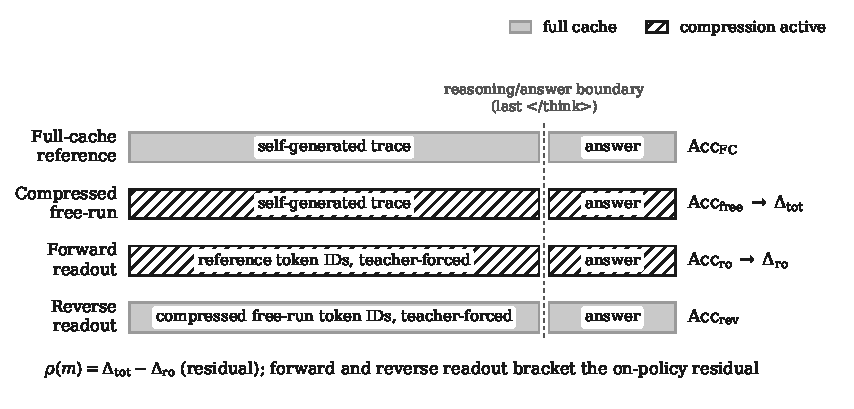
\includegraphics[width=0.92\linewidth]{figures/fig0_protocol.pdf}
\caption{The four generation protocols behind the estimands. Fill encodes the cache condition while a span is processed (grey $=$ full cache; hatched $=$ compression active); the text in each span says where its tokens come from (self-generated versus teacher-forced replay of exact stored token IDs). Forward readout scores answer generation \emph{under compression} given the full-cache reference trace; reverse readout scores \emph{full-cache} answer generation given the compressed model's own trace. The residual $\res{m} = \dtot{m} - \dro{m}$ is the free-running loss unexplained by on-reference readout; the forward and reverse estimates bracket the on-policy residual (\cref{sec:reverse}).}
\label{fig:protocol}
\end{figure}

\begin{definition}[Total change]
$\accfree{m}$ is the accuracy of free-running generation with compression active throughout. The total change is
\begin{equation}
\dtot{m} \;=\; \accfree{m} - \accfc .
\end{equation}
\end{definition}

\begin{definition}[On-reference (forward) readout]
For each FC reference trace, the reasoning/answer boundary is deterministic and logged per row: the \emph{last} \texttt{</think>} token when present (robust to multiple closes and \texttt{\textbackslash boxed\{\}} emitted mid-reasoning); else an answer-marker fallback; else \emph{undefined}. Undefined-boundary rows are excluded from readout accuracy and counted ($n_{\mathrm{readout\text{-}undefined}}$), never silently dropped. The exact stored reference token IDs are teacher-forced through the boundary into the \emph{compressed} cache; from the boundary, the answer span is freely sampled under the same compression method, budget, temperature, top-$p$, and matched seed, and scored with the frozen grader. This yields $\accro{m}$ and
\begin{equation}
\dro{m} \;=\; \accro{m} - \accfc .
\end{equation}
\end{definition}

\begin{definition}[Residual --- a definition, not a measured cause]
\begin{equation}
\res{m} \;=\; \dtot{m} - \dro{m} \;=\; \accfree{m} - \accro{m}.
\label{eq:residual}
\end{equation}
$\res{m}$ is labeled, throughout, \emph{accuracy change unexplained by on-reference readout}. It is not a directly measured causal effect of trajectory distortion. Because the readout intervention conditions on the good full-cache trajectory, it plausibly underestimates readout failure on the states the compressed model actually visits, biasing $\res{m}$ toward the trajectory share (the covariate-shift argument of~\cite{ross2011dagger}). This caveat is structural to the estimand and is stated here, up front.
\end{definition}

\begin{definition}[Reverse readout and the residual bracket]
Reverse readout inverts the roles: the \emph{compressed free-run} trace is teacher-forced to its boundary under the \emph{full} cache, and the answer span is generated full-cache, yielding $\accrev{m}$. Both bracket endpoints are $\text{total} - \text{readout}$ residual estimates, with the readout change measured on two different state distributions: the forward endpoint $\rho_{\mathrm{fwd}} = \dtot{m} - \dro{m}$ measures readout on \emph{reference} states, and the reverse endpoint measures it on the compressed model's \emph{own} states, since $\accfree{m} - \accrev{m}$ is the cost of compressed versus clean readout of the same compressed traces:
\begin{gather}
\rho_{\mathrm{rev}}(m) \;=\; \dtot{m} - \bigl(\accfree{m} - \accrev{m}\bigr) \;=\; \accrev{m} - \accfc ,\\
\rho_{\mathrm{bracket}}(m) \;=\; \bigl[\, \min(\rho_{\mathrm{fwd}}, \rho_{\mathrm{rev}}),\; \max(\rho_{\mathrm{fwd}}, \rho_{\mathrm{rev}}) \,\bigr].
\end{gather}
The two estimates are off-policy in opposite directions, so their interval brackets the on-policy residual. A bracket bounded away from zero is what licenses the (bounded) causal reading of the residual; the point estimate alone does not.
\end{definition}

\begin{definition}[ADD: answer-distribution distortion]
For each problem, let $P_{\mathrm{FC}}$ and $P_m$ be the coarsened, canonicalized answer distributions over the FC bank ($n{=}8$) and the compressed cell ($n{=}4$; the TV estimate's variance is dominated by the smaller $n$, so the asymmetry only tightens the reference side). Then
\begin{equation}
\ADD(m) \;=\; \TV\bigl(P_{\mathrm{FC}}, P_m\bigr),
\end{equation}
a \emph{lower bound} on behavioral change --- it sees only changes that reach the answer --- and never described as ``behavioral change'' tout court. ADD is reported alongside its two channels: the \textbf{termination-mass shift} (signed change in \texttt{OTHER}/truncation-bucket probability; a length effect) and the \textbf{within-answered TV} (TV between the \emph{renormalized} answered-only distributions; the reasoning channel) --- these are separate diagnostics, not additive parts of ADD --- so a truncation increase is never read as a reasoning change; the identity $\ADD \ge \tfrac{1}{2}\lvert \text{termination shift} \rvert$ is reported. Significance uses a per-problem exact or Monte Carlo \textbf{permutation null} formed by relabeling pooled samples (split-half subtraction is prohibited), with Benjamini--Hochberg correction across problems. Every ADD value is accompanied by its \textbf{signed flip-mass} --- gained versus lost correct-answer mass --- because divergence from the reference is not intrinsically damage; correctness is the arbiter.
\end{definition}

\begin{definition}[TV profile and onset]
Per-step divergence between full-cache and compressed \emph{teacher-forced replay} of the same token IDs is measured as total variation between next-token distributions, $\TV_t = \TV\bigl(p^{\mathrm{FC}}_t, p^{m}_t\bigr)$ --- TV, not KL, for the speculative-decoding behavioral reading noted above. Profiles are onset-aligned at each row's first prune event; summaries are threshold-free AUC-TV and windowed means (pre-eviction, first 50 post-eviction steps, later steps). These are distribution-fidelity instruments on their own scale; they are never subtracted from an accuracy delta.
\end{definition}

\subsection{Pre-registration}
The decomposition's read was pre-committed before the powered numbers existed, with named \textsc{confirm} / \textsc{complicate} / \textsc{refute} criteria (CI-based thresholds on readout accuracy, readout share, and share separability), and we report the outcome whatever it shows. The outcome was \textsc{complicate} (\cref{sec:forward}). The pilot double dissociation that motivated the confirmatory criteria was itself pre-registered as an unconfirmed, hypothesis-generating observation from $n{=}5$ problems. Deviations from the original protocol are recorded in the pre-registration's dated, append-only amendment log; the material one is cell size --- the original specification named 250 problems $\times$ $n{=}8$ for compression cells, and the powered cells ran at 100 $\times$ $n{=}4$ (fixed, with the pre-committed read, before the decisive readout run) --- with the full-cache reference kept at 250 $\times$ $n{=}8$.

% =====================================================================
\section{Results}
\label{sec:results}

All compression-cell results are at budget 256 on MATH-500 unless stated; confidence intervals are problem-clustered bootstrap 95\% CIs against the single pinned FC reference. \textsc{Done} items are final; the scale-axis cells (R1-Distill-Qwen-1.5B/-14B, Amendment J) are \emph{in progress} and appear only in \cref{sec:threats,sec:conclusion} as planned extensions.

\subsection{The powered phenomenon: collapse, and random beats recency}
\label{sec:phenomenon}
From $\accfc = 0.882$, free-running accuracy at budget 256 falls to $\mathbf{0.237}$ for StreamingLLM and $\mathbf{0.422}$ for Random (100 problems $\times$ 4 seeds per cell). Random eviction beats the principled sinks-plus-recency policy by $+0.185$, 95\% CI $[0.130, 0.242]$; the per-problem difference is non-negative on \textbf{94/100 problems} (44 strict wins, 50 ties --- mostly problems both methods jointly solve or jointly fail --- and 6 losses). The H2O-style press lands at StreamingLLM's level ($0.247$; \cref{tab:decomp}), so at this budget the uniform floor beats \emph{both} principled allocations --- positional and attention-score. The collapse is a \emph{budget} effect, not an artifact of free-running under our harness: at budget 2048 the same presses free-run at $0.850$ (Random) and $0.807$ (StreamingLLM) --- within $0.03$--$0.07$ of the reference (800/800 conditions; the full 2048 decomposition is in \cref{sec:forward}) --- and the Random$>$StreamingLLM ordering persists ($+0.042$). Both presses retain the same total budget (\cref{sec:setup}), so the gap is \emph{which} 256 tokens are kept, not how many. HOTT itself carries no random-eviction baseline, so this comparison is not available there; concurrent method work points in the same direction --- value-aware \emph{stochastic} eviction reports higher reasoning accuracy than deterministic selection-based baselines, attributing the gain to eviction diversity~\cite{vase2026}. This is the phenomenon the rest of the paper decomposes: free-running degradation of the kind HOTT reports --- sharpest, as in HOTT, for StreamingLLM --- at a compression level the method literature certifies as safe under readout-shaped evaluation.

\begin{figure}[t]
\centering
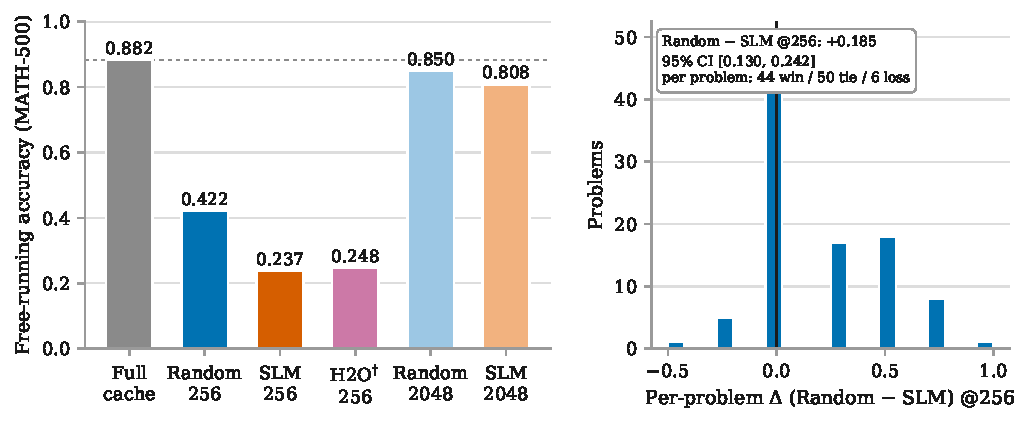
\includegraphics[width=0.9\linewidth]{figures/fig1_phenomenon.pdf}
\caption{Left: free-running accuracy by method and budget --- the collapse is a budget effect (full cache $0.882$; at 256, Random $0.422$ / StreamingLLM $0.237$ / H2O-style$^{\dagger}$ $0.247$ / R-KV$^{\ddagger}$ $0.520$; at 2048, $0.850$ / $0.807$ / $0.823$, the near-lossless pole; light tints $=$ budget 2048; $\dagger$, $\ddagger$ per \cref{tab:decomp}). Even the best policy at 256, the reasoning-specific R-KV, loses $0.36$ of the reference accuracy. Right: per-problem paired differences at budget 256 --- Random $-$ StreamingLLM is $+0.185$ on average (95\% CI $[0.130, 0.242]$) and non-negative on 94/100 problems (44 strict wins, 50 ties, 6 losses).}
\label{fig:phenomenon}
\end{figure}

\subsection{Forward decomposition: the loss is mostly not readout}
\label{sec:forward}
\cref{tab:decomp} gives the forward decomposition: 400 conditions per cell (100 problems $\times$ 4 seeds), four method cells.

\begin{table}[t]
\centering
\caption{Forward decomposition at budget 256 (400 conditions per cell: 100 problems $\times$ 4 seeds). $\accfc = 0.882$. CIs are problem-clustered bootstrap 95\% (2000 resamples, percentile). Readout share $= \dro{m}/\dtot{m}$ (ratio of cell means). Trunc.\ = per-cell truncation rate; truncated rows remain in every denominator, scored incorrect. Undefined reasoning/answer boundary: 8 rows per cell, balanced across methods.}
\label{tab:decomp}
\footnotesize
\setlength{\tabcolsep}{4pt}
\begin{tabular}{lccccccc}
\toprule
Method @256 & $\accfree{m}$ (95\% CI) & $\accro{m}$ (95\% CI) & $\dtot{m}$ & $\dro{m}$ & $\res{m}$ & Readout share & Trunc. \\
\midrule
Random       & 0.422 $[0.343, 0.500]$ & 0.765 $[0.686, 0.817]$ & $-0.460$ & $-0.117$ & $\mathbf{-0.343}$ & 25\% & 0.233 \\
StreamingLLM & 0.237 $[0.172, 0.302]$ & 0.584 $[0.495, 0.647]$ & $-0.645$ & $-0.298$ & $\mathbf{-0.347}$ & 46\% & 0.070 \\
H2O-style$^{\dagger}$ & 0.247 $[0.180, 0.318]$ & 0.597 $[0.503, 0.668]$ & $-0.635$ & $-0.286$ & $\mathbf{-0.349}$ & 45\% & 0.105 \\
R-KV$^{\ddagger}$ & 0.520 $[0.435, 0.610]$ & 0.798 $[0.710, 0.850]$ & $-0.362$ & $-0.084$ & $\mathbf{-0.278}$ & 23\% & 0.135 \\
\bottomrule
\end{tabular}

\smallskip
{\footnotesize $^{\dagger}$kvpress \texttt{ObservedAttentionPress}: the accumulated-attention heavy-hitter signal \emph{without} the original H2O's recent-window reservation (\cref{sec:setup}); eager attention, generation capped at 8192 tokens (eager-kernel memory), truncations in-denominator as always.}

{\footnotesize $^{\ddagger}$our R-KV port, parity-verified against the authors' code (retained-set Jaccard $1.0$) and smoke-verified during decoding (\cref{sec:control}); 16384-token cap like Random/StreamingLLM. Numbers characterize the certified port at 7B, not the authors' setup.}
\end{table}

Two facts carry the paper. \textbf{(i) A large trajectory residual exists for every policy tested.} Readout accuracy sits far above free-running accuracy for all three presses (non-overlapping with the free-run values), leaving residuals of $-0.343$, $-0.347$, and $-0.349$: roughly 34 accuracy points --- for three \emph{mechanistically unrelated} selection rules (uniform, positional, attention-score) --- that held-fixed-trace accuracy evaluation does not register. A protocol that teacher-forces the reasoning trace and scores answer readout would certify Random-256 at $0.765$ --- within sight of the $0.882$ reference --- while its deployed free-running accuracy is $0.422$. This is, in one row of a table, the resolution of the near-lossless/collapse contradiction. Nor is the residual a truncation artifact: scoring every truncated free-run as \emph{correct} still leaves residuals of $-0.110$ (Random) and $-0.277$ (StreamingLLM) --- and that bound is extreme by construction, since it scores as successes the very termination failures ADD measures as a compression-induced channel (\cref{sec:add}). \textbf{(ii) The method differences live in the readout channel.} The $+0.185$ Random-vs-StreamingLLM free-run gap decomposes into a $0.181$ difference in readout change and a $0.004$ difference in residual, and the pattern generalizes: across all three policies the forward residuals span $0.006$ ($-0.343$ to $-0.349$, CIs mutually overlapping and all excluding zero) while the readout changes span $0.169$ ($-0.117$ to $-0.286$). On the forward estimand, a residual of similar magnitude exists for \emph{every} policy tested; what a policy chooses to keep decides how well the trace can be read out, not how far the freely written trace drifts. We still report this cross-policy similarity as \textbf{exploratory} (one model, one benchmark, one budget; and the reverse-side residual estimates do separate Random from StreamingLLM, \cref{sec:reverse}). Truncation rates differ sharply --- Random $0.233$ versus StreamingLLM $0.070$, a $3.3\times$ gap --- and, with truncations in-denominator and scored incorrect, this anticipates Random's larger ADD termination-mass shift ($+0.224$ vs.\ $+0.081$; \cref{sec:add}).

\textbf{R-KV: the reasoning-specific policy free-runs best, and still carries the structure.} Our parity- and smoke-verified R-KV port (\cref{sec:control}) is the strongest free-runner at budget 256 --- $0.520$ against Random's $0.422$ --- directionally consistent with its redundancy-aware design. The decomposition finds the same shape regardless: readout $0.798$ (within sight of the $0.882$ reference) against free-running $0.520$, a residual of $-0.278$ (CI $[-0.335, -0.195]$) --- nominally smaller than the $-0.34$ trio, with overlapping CIs, so we claim neither that the four residuals are equal nor that R-KV's separates. The operative point survives the best policy tested: a held-trace protocol would certify it at $0.798$ while it deploys at $0.520$. These numbers characterize our certified port at 7B, not the authors' setup (\cref{sec:threats}).

\textbf{Why does random beat recency? (hypothesis-level.)} We offer an interpretation, explicitly labeled as unverified: StreamingLLM's sinks-plus-recent-window allocation discards the early portion of the trace --- the problem statement and its givens --- which is precisely the material answer readout needs to consult, whereas uniform random eviction preserves a coarse, thinned sketch of the \emph{entire} trajectory, problem statement included. This interpretation is consistent with where the gap localizes --- entirely in the readout channel --- but no eviction-content attribution experiment in this paper tests it; we advance it as hypothesis, not finding.

\textbf{Dose response: the residual shrinks with budget.} At budget 2048 the same decomposition (400 conditions per cell) yields readout accuracies of $0.901$ (95\% CI $[0.820, 0.943]$) and $0.903$ ($[0.823, 0.943]$) --- statistically indistinguishable from, and nominally above, the $0.882$ reference --- against free-running $0.850$ (Random) and $0.807$ (StreamingLLM): trajectory residuals of $-0.051$ (CI $[-0.065, -0.010]$) and $-0.096$ ($[-0.128, -0.043]$), a factor of $3.6$--$6.8$ below the $-0.34$ residuals at 256. The H2O-style press behaves alike ($0.823$ free, $0.898$ readout, residual $-0.075$, CI $[-0.102, -0.020]$), so the dose response holds for all three policies. With readout lossless at this budget, the residual is no longer merely the larger channel --- it is effectively the \emph{entire} remaining loss. The trajectory channel is a low-budget phenomenon in magnitude, not in kind: at 3.8\% of the mean trace it dominates a collapse; at 56.6\% it shrinks to a small fraction of the reference gap, with CIs still excluding zero. A direct control calibrates the readout protocol itself: full-cache readout of the full-cache reference traces --- zero compression anywhere --- scores $0.906$ against the $0.882$ reference (400 conditions), putting the pure answer-resampling effect at $+0.023$: an order of magnitude below the residuals at 256, and in the direction that \emph{shrinks} them, so answer-resampling easiness cannot manufacture the residual.

\textbf{Pre-registered outcome: \textsc{complicate}.} The pre-committed criteria for the strong headline required Random to be readout-lossless (readout CI lower bound $\ge 0.75$) and the two readout shares to separate with StreamingLLM $\ge 0.5$. Neither held: Random's readout change is significantly negative (CI lower bound $0.686 < 0.75$) and StreamingLLM's share is $0.46 < 0.5$. The pilot's clean ``StreamingLLM$=$readout-dominated, Random$=$trajectory-dominated'' double dissociation is therefore \emph{false} at power; reality is ``both heavily and equally trajectory-damaged, differing in readout fidelity.'' The central residual --- the part the contradiction needs --- confirmed robustly; the paper is framed around what survived.

\subsection{Reverse-replay bracket: the residual survives the off-policy correction}
\label{sec:reverse}
The forward residual conditions on full-cache states and is biased toward the trajectory share (\cref{eq:residual}). Reverse replay measures the residual from the other side: the compressed free-run trace is read out under the \emph{full} cache. If the free-running loss were mostly readout failure that the forward estimand mis-assigns, clean full-cache readout of the compressed trajectory would recover accuracy toward $\accfc$. It does not: $\accrev{\text{Random}} = 0.636$, $\accrev{\text{SLM}} = 0.417$, $\accrev{\text{H2O-style}} = 0.419$, and $\accrev{\text{R-KV}} = 0.662$ versus $\accfc = 0.882$ (400 reverse-readout conditions per cell; defined answer boundaries: 308 / 372 / 360 / 346). A large part of the loss is genuinely in the trajectory: the compressed model has, by the time it reaches its answer, written itself into reasoning states from which even an uncompressed reader cannot recover the correct answer.

The resulting residual brackets are \textbf{Random $[-0.343, -0.246]$}, \textbf{StreamingLLM $[-0.466, -0.347]$}, \textbf{H2O-style $[-0.463, -0.349]$}, and \textbf{R-KV $[-0.278, -0.221]$} --- never near zero. Problem-clustered bootstrap 95\% CIs on all eight endpoints exclude zero: forward $[-0.402, -0.258]$ / $[-0.403, -0.268]$ / $[-0.403, -0.270]$ / $[-0.335, -0.195]$; reverse $[-0.383, -0.213]$ / $[-0.553, -0.410]$ / $[-0.566, -0.420]$ / $[-0.355, -0.203]$. The central claim (a large, readout-invisible trajectory residual) \emph{survives} the off-policy correction for all four policies, with statistical significance at every endpoint.

Three honest qualifications. First, the anticipated bias ordering --- forward inflates the residual, reverse deflates it --- holds for Random but \emph{reverses} for both concentrated policies, so the intervals are reported as min/max brackets of the two estimates, not as directional bias bounds.

Second, the two sides disagree on method structure, and the endpoint CIs quantify the disagreement: the forward endpoints of the original trio are statistically indistinguishable, while the reverse endpoints split \emph{recoverable from concentrated} --- StreamingLLM and H2O-style land together ($-0.466$ and $-0.463$, CIs overlapping) and separate with non-overlapping CIs from both Random ($-0.246$) and R-KV ($-0.221$), whose reverse CIs overlap each other. The concentrated policies write confidently wrong reasoning that even a clean reader cannot rescue (consistent with StreamingLLM's within-answered ADD profile, \cref{sec:add}); uniform and redundancy-aware eviction leave traces that stay more recoverable. Because the attribution is \emph{estimand-dependent} --- invariant on the forward side, structured on the reverse side --- we still do not claim a single method-level readout-vs-trajectory attribution; we report the central residual strongly and the reverse-side structure as significant but exploratory.

Third, undefined-boundary reverse rows could be \emph{informative} missingness: a rambling trace that never reaches an answer boundary is plausibly a worse trajectory, and the policies differ in how many they produce (92 / 28 / 40 / 54 of 400), so excluding them could bias $\accrev{m}$ upward. We bound this selection effect by imputation. Scoring every undefined-boundary row as \emph{incorrect} gives reverse endpoints of $-0.392$ / $-0.495$ / $-0.505$ / $-0.310$; scoring every one as \emph{correct} gives $-0.162$ / $-0.425$ / $-0.405$ / $-0.175$. Under \emph{any} imputation, the residual bracket excludes zero for every policy (at worst, Random's bracket widens to $[-0.343, -0.162]$) --- the selection effect cannot manufacture the residual.

\begin{figure}[t]
\centering
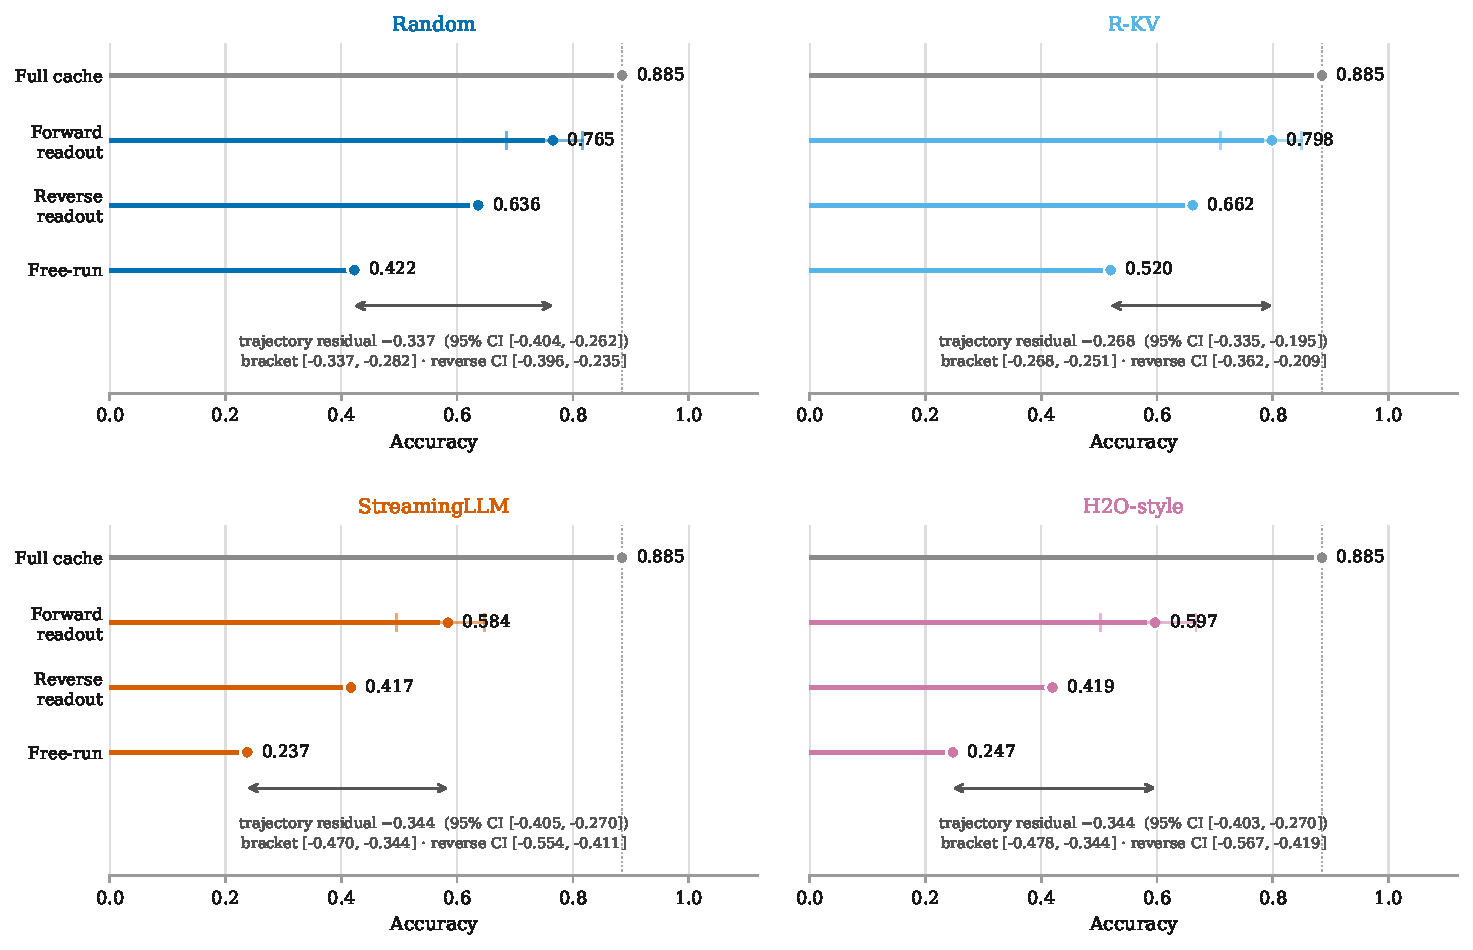
\includegraphics[width=0.9\linewidth]{figures/fig2_bracket.pdf}
\caption{Accuracy ladders from the full-cache reference ($0.882$) down through forward readout, reverse readout, and free-run, per policy --- top row the \emph{recoverable} pair (Random, R-KV), bottom row the \emph{concentrated} pair (StreamingLLM, H2O-style), the reverse-side split of \cref{sec:reverse}. The arrow marks the forward trajectory residual (the free-run--to--readout gap); whiskers on the forward-readout rung are its problem-clustered 95\% accuracy CI. The residual brackets (Random $[-0.343, -0.246]$, R-KV $[-0.278, -0.221]$, StreamingLLM $[-0.466, -0.347]$, H2O-style $[-0.463, -0.349]$) and the 95\% CIs on all eight endpoints (beneath each panel) exclude zero: even the best free-runner leaves a large, readout-invisible residual, and the concentrated policies' traces resist even clean full-cache readout.}
\label{fig:bracket}
\end{figure}

\subsection{The mechanism: divergence is zero at eviction and compounds}
\label{sec:mechanism}
Why does readout-style evaluation miss a 34-point loss? \cref{fig:tvprofile} answers with onset-aligned per-step TV between full-cache and compressed teacher-forced replay of identical token IDs (800 profiles; median onset at step 65, one step after the first prune at the compression interval of 64).

\begin{table}[t]
\centering
\caption{Onset-aligned per-step TV between full and compressed teacher-forced replay (800 profiles). Entries are means of per-trace window means (each trace counts once, matching the problem-clustered convention); the step-pooled later-window mean is \emph{larger} ($0.118$), because longer traces diverge more.}
\label{tab:tv}
\begin{tabular}{lc}
\toprule
Window relative to first eviction & Mean per-step TV \\
\midrule
Before eviction & $\mathbf{0.0000}$ \\
First 50 steps after & $0.0018$ \\
Later steps ($>$50 after) & $\mathbf{0.0884}$ \\
\bottomrule
\end{tabular}
\end{table}

\begin{figure}[t]
\centering
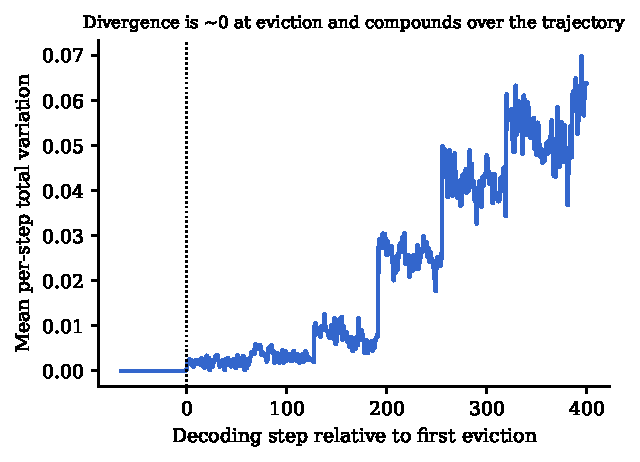
\includegraphics[width=0.72\linewidth]{figures/fig4_tvprofile.pdf}
\caption{Onset-aligned mean per-step TV over 800 replay profiles: exactly zero before the first eviction, near-zero immediately after, then a compounding staircase whose steps align with eviction events (every 64 decoding steps) --- slow drift, not an instantaneous readout error. The curve is shown to $+400$ steps of onset; the later-steps windowed mean of $0.0884$ (\cref{tab:tv}, per-trace estimator; step-pooled $0.118$) covers the full horizon, where divergence continues to grow.}
\label{fig:tvprofile}
\end{figure}

Three readings. First, the \textbf{mechanism}: the divergence induced by eviction is near-zero \emph{at the moment it happens} ($0.0018$ per step over the next 50 steps) and grows by roughly $50\times$ over the remaining trajectory --- a slow-compounding drift. Note the a-fortiori structure of this measurement: the profile is computed under teacher forcing, with the trace held fixed, so the compounding reflects accumulating cache-state divergence alone, with \emph{no} feedback through sampled tokens; free-running generation adds a second divergence source on top of this --- feedback through the model's own sampled outputs. Any single-step or short-horizon evaluation therefore measures the $\approx 0.002$ pre-compounding regime, and accuracy-scale readout evaluation registers only the distortion present at answer time --- not the counterfactual rewriting of the trajectory that free-running generation exposes; this is the quantitative form of the paper's thesis. Second, \textbf{the forward similarity corroborated}: AUC-TV is matched across all three policies ($0.086$ Random, $0.083$ StreamingLLM, $0.073$ H2O-style over its 400 profiles, median onset likewise 65), consistent with the similar-magnitude forward residuals of \cref{sec:forward} (exploratory; the reverse-side estimates separate, \cref{sec:reverse}). Third, \textbf{instrument validity}: the exactly-zero pre-eviction TV doubles as a self-control --- the replay harness introduces no divergence of its own.

\subsection{ADD: silent answer-distribution distortion, with signed flips}
\label{sec:add}
Accuracy alone understates what compression does to the answer distribution. \cref{tab:add} reports ADD with its channel diagnostics and, per our direction discipline, the signed flip-mass.

\begin{table}[t]
\centering
\caption{Answer-distribution distortion at budget 256. Within-answered TV is over renormalized answered-only distributions (a channel diagnostic, not an additive part of ADD). Signed flip-mass is net gained-minus-lost correct-answer mass; all four policies are overwhelmingly on the losing side. ADD values far exceed the $\approx 0.07$ negative-control noise floor (\cref{sec:control}).}
\label{tab:add}
\footnotesize
\begin{tabular}{lcccc}
\toprule
Method & Mean ADD & Within-answered TV & Termination shift & Signed flip-mass (net) \\
\midrule
StreamingLLM & 0.751 & 0.749 & $+0.081$ & $-0.646$ \\
H2O-style    & 0.715 & 0.713 & $+0.101$ & $-0.636$ \\
Random       & 0.559 & 0.504 & $+0.224$ & $-0.461$ \\
R-KV         & 0.459 & 0.450 & $+0.149$ & $-0.364$ \\
\bottomrule
\end{tabular}
\end{table}

The decomposition separates two failure styles that headline accuracy conflates, and the split again follows the recoverable-vs-concentrated line of \cref{sec:reverse}. Both concentrated policies are almost entirely \emph{within-answered} (StreamingLLM $0.749$ of ADD $0.751$; H2O-style $0.713$ of $0.715$, with zero gained flip-mass): they keep producing confident answers, but different, wrong ones --- silent flips. Random carries a much larger \emph{termination-mass} shift ($+0.224$): it rambles and fails to terminate, consistent with its higher truncation rate (truncations remain in all denominators, scored incorrect). The certified R-KV port completes the picture coherently: the lowest ADD of the four ($0.459$, still ${\sim}7\times$ the noise floor), with the second-largest termination shift ($+0.149$; truncation $0.135$) and flip-mass again overwhelmingly toward lost correct answers ($-0.364$; gained $0.004$) --- less distribution damage, in step with its higher accuracy, and no denoising. So even where the two methods' accuracies were similar, they would damage the answer distribution through different channels --- a distinction invisible to pass@1. The signed flip-mass ($-0.646$ and $-0.461$ net toward lost correct answers) is what licenses reading this divergence as loss rather than mere change: on these cells, deviation from the reference is not denoising. HOTT independently observes that eviction makes reasoning models ``more talkative, generating longer sequences''~\cite{hott2025} --- external corroboration of the termination-mass/truncation channel we measure most strongly for Random. The instrument also scales coherently with budget: at 2048, mean ADD falls to $0.085$ (Random; approaching the $0.068$ two-FC floor) and $0.146$ (StreamingLLM; ${\approx}2\times$ the floor, net flip $-0.076$), so distribution distortion tracks the dose --- we observe only modest answer churn beyond the accuracy change at the near-lossless pole, and we report this against our pre-registered silent-flip hypothesis honestly: the large-ADD-at-flat-accuracy regime did not materialize at 2048.

\begin{figure}[t]
\centering
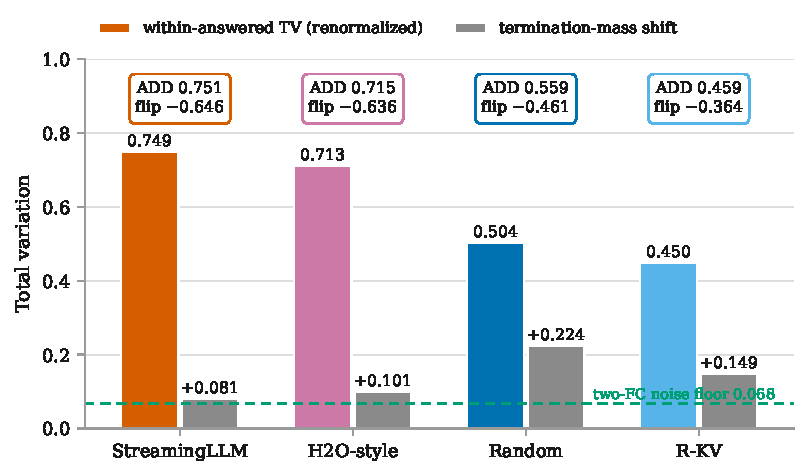
\includegraphics[width=0.72\linewidth]{figures/fig3_add.pdf}
\caption{Two failure styles that headline accuracy conflates, split along the recoverable-vs-concentrated line: both concentrated policies are nearly all within-answered (StreamingLLM $0.749$ of ADD $0.751$; H2O-style $0.713$ of $0.715$) --- silent answer flips --- while Random and R-KV carry larger termination-mass shifts ($+0.224$ and $+0.149$). R-KV's ADD is the lowest of the four ($0.459$), coherent with its highest free-running accuracy; flip-mass is overwhelmingly toward lost correct answers for all four. Dashed line marks the two-FC noise floor ($0.068$).}
\label{fig:add}
\end{figure}

\subsection{Negative control: the instrument does not false-positive}
\label{sec:control}
Splitting the FC bank into two disjoint four-seed halves and running the full ADD pipeline between them yields \textbf{mean ADD $0.068$, median $0.000$, mean permutation $p = 0.976$, and $0\%$ of problems significant} ($n = 250$). The noise floor of the instrument ($\approx 0.07$) sits $7$--$11\times$ below the compression cells ($0.46$--$0.75$ across the four policies, \cref{tab:add}): ADD does not light up on null data. Per our pre-registration this control is presented as a figure, not a sentence.

\begin{figure}[t]
\centering
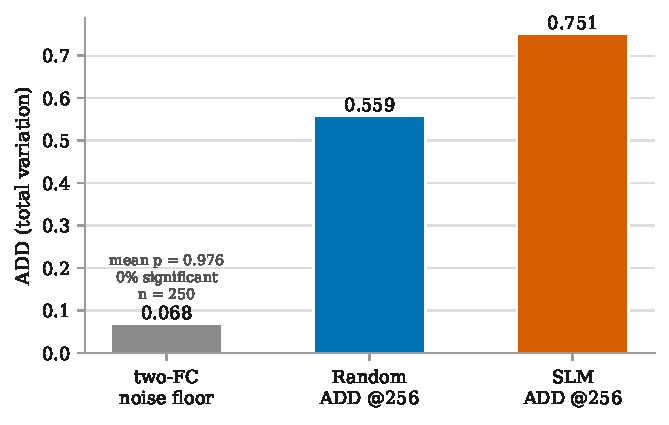
\includegraphics[width=0.72\linewidth]{figures/fig5_twofc.pdf}
\caption{Two-full-cache negative control ($n = 250$): ADD between disjoint FC seed halves has mean $0.068$ (median $0.000$, mean permutation $p = 0.976$, $0\%$ of problems significant), far below the compression cells (Random $0.559$ and StreamingLLM $0.751$ shown; all four policies lie in $0.46$--$0.75$, \cref{tab:add}) --- the instrument does not false-positive.}
\label{fig:control}
\end{figure}

A second validity artifact gated the R-KV cells: our R-KV port reproduces the authors' retained-token sets \emph{exactly} (Jaccard $1.0$ at budgets $\{128, 256, 384, 512\}$ on synthetic tensors) --- a mechanism-level match, which is the test that catches a subtly wrong port. The pre-registered real-generation smoke then also passed (retained-set Jaccard $1.0000$ against the live press during decoding), and only after both gates did R-KV rows enter analysis (\cref{tab:decomp}).

% =====================================================================
\section{Threats to Validity}
\label{sec:threats}

We treat this section as part of the paper's evidence, not as an apology: each threat is paired with the specific control that bounds it.

\textbf{Generality (the primary threat).} All headline decomposition results are one primary model (DeepSeek-R1-Distill-Qwen-7B; subset-scale Llama-base check below), one benchmark (MATH-500), one primary budget (256, with a completed 2048 dose-response decomposition, \cref{sec:forward}), four eviction policies. The cross-policy similarity of the trajectory residual and any generality claim remain \emph{exploratory} on the other axes. \emph{Control:} the claims are scoped accordingly throughout, and the widening grid is landing: the budget-2048 decomposition is complete --- readout statistically indistinguishable from the reference, small residuals with CIs excluding zero (\cref{sec:forward}); the H2O-style decomposition is now fully \emph{in} --- forward (\cref{tab:decomp}), reverse bracket (\cref{sec:reverse}), 2048 dose point (\cref{sec:forward}), and divergence profiles (\cref{sec:mechanism}) --- and we note this press is the heavy-hitter signal \emph{without} H2O's recent-window reservation, so its free-running collapse neither reproduces nor contradicts HOTT's H2O result (what it adds is that an attention-score policy carries the same trajectory residual as positional and uniform ones); the R-KV cells cleared their two-stage integrity gate (retained-set parity, then a real-generation smoke) and are in (\cref{tab:decomp}); the cross-architecture check is in (next paragraph); AIME-24 is queued. The pre-registered analysis was fixed before any of these cells completed.

\emph{Cross-architecture check (subset scale).} On DeepSeek-R1-Distill-Llama-8B (50 problems $\times$ 4 seeds per cell against its own pinned reference bank, $\accfc = 0.805$; CIs correspondingly wider), the central result replicates on the paper's sharpest case: StreamingLLM-256 free-runs at $0.235$ against readout $0.508$ --- residual $-0.273$ (CI $[-0.345, -0.175]$), bracket $[-0.426, -0.273]$, reverse CI $[-0.523, -0.327]$, zero excluded throughout. The readout-invisible trajectory residual is not an artifact of the Qwen lineage. Random-256, by contrast, enters a \emph{degenerate} regime on the Llama base: free-running accuracy $0.000$ with truncation $0.805$ --- the traces collapse into non-terminating filler rather than reasoning, consistent with the Llama family's attention-sink sensitivity~\cite{xiao2023streamingllm} (uniform eviction removes the sink tokens that the sinks-plus-recency policy preserves) --- and readout falls to $0.021$, so both channels floor and the decomposition is uninformative for that cell (residual $-0.021$, bracket $[-0.021, 0.028]$ spanning zero; 6 of 400 reverse rows reach an answer boundary). Two boundaries follow, reported plainly: the budget-256 random-beats-recency ordering is architecture-dependent --- it \emph{reverses} on the Llama base ($0.000$ vs.\ $0.235$) --- and a near-zero residual at floor accuracy is not evidence of a small trajectory channel; there is no accuracy left to attribute.

\textbf{No $>$100\% regime observed.} We saw no accuracy gains under compression on small-budget MATH-500 --- including from our certified R-KV port (gained flip-mass $0.0025$ at budget 256, \cref{tab:decomp}). \emph{Control:} the framing carries no denoising claim anywhere --- title, thesis, and headline are strictly near-lossless-under-readout versus collapse-under-free-generation. R-KV's published claim --- $105\%$ of full-KV accuracy at ${\sim}16\%$ cache on AIME-24 with R1-Distill-Llama-8B, a $>$100\% regime at another model scale, and notably established with \emph{free-running} evaluation (\cref{tab:audit}) --- was tested directly. On AIME-24 at budget 2048 ($19.7\%$ of the mean 10{,}415-token trace; own pinned reference bank, $\accfc = 0.371$ with $0.221$ truncation under the 16384 cap; 30 problems $\times$ 4 seeds), no press exceeded the reference: best free-run $0.283$ (Random), our certified R-KV port $0.217$, StreamingLLM $0.142$; gained flip-mass at most $0.050$. At 7B, in our protocol, the $>$100\% regime did not appear --- per Amendment E a finding about scale and protocol, not a port failure (retained sets match the authors' code exactly). The decomposition replicates on this second benchmark: forward residuals $-0.179$ / $-0.246$ / $-0.321$ (Random / R-KV / StreamingLLM) with problem-clustered CIs $[-0.349, -0.076]$ / $[-0.419, -0.139]$ / $[-0.509, -0.202]$, all excluding zero. The readout channel also makes the paper's point in its sharpest form yet: all three presses read out at an \emph{identical} $0.462$ ($[0.327, 0.661]$) --- 85 of 93 defined rows converge to the same extracted answer through visibly different generations, and on the 8 divergent rows every press is wrong --- so held-trace evaluation literally cannot distinguish policies that free-running separates by $2\times$ (\cref{fig:aime}).

\begin{figure}[t]
\centering
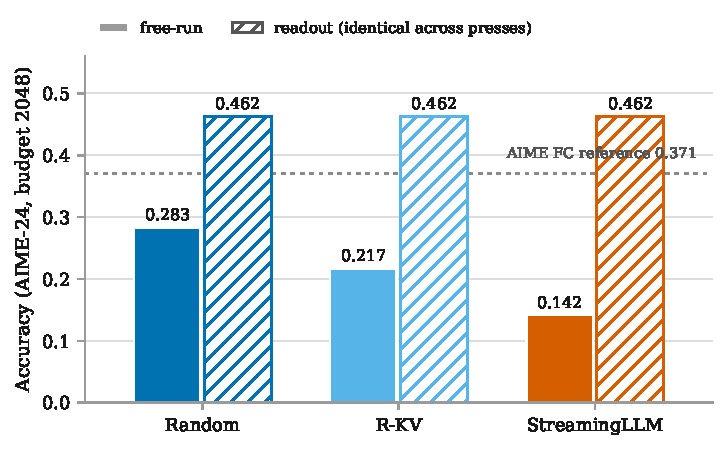
\includegraphics[width=0.6\linewidth]{figures/fig6_aime.pdf}
\caption{AIME-24 at budget 2048 (subset scale: 30 problems $\times$ 4 seeds; own reference bank at $0.371$). Free-running separates the three policies ($0.283$ / $0.217$ / $0.142$); their readout accuracies are \emph{identical} at $0.462$ --- same correctness on every one of 120 conditions, with 85 of 93 defined rows converging to the same extracted answer through visibly different generations. Held-trace evaluation cannot see the difference between these policies at all; no press approaches the reference (no $>$100\% regime).}
\label{fig:aime}
\end{figure}

\textbf{Off-policy bias of the residual.} The forward residual conditions on full-cache states and is biased toward the trajectory share; this is stated at the definition (\cref{eq:residual}), not held for rebuttal. \emph{Control:} the reverse-replay bracket \emph{bounds} the bias --- it does not eliminate it --- and the bracket excludes zero for all three policies, with problem-clustered bootstrap CIs on all six endpoints excluding zero (\cref{sec:reverse}). The honest costs of the bracket are also stated: the anticipated bias ordering reverses for both concentrated policies, and the method-level split is estimand-dependent, so it is reported only as bracketed and exploratory. The differential defined-reverse counts (308 / 372 / 360) are bounded by imputation (\cref{sec:reverse}): under any scoring of the undefined-boundary rows, the bracket excludes zero for every policy. A related objection --- that teacher-forced readout is ``easy by construction'' because the reference trace already contains the answer-relevant work --- is not a confound but the finding: the held-trace evaluation protocols that certify compression methods share exactly this easiness, and the reverse direction extends the same easiness to the compressed trace without recovering accuracy.

\textbf{Kernel confound.} H2O's attention-score press requires eager attention while the other presses run under sdpa, whose numerics differ. \emph{Control:} full-cache accuracy under eager versus sdpa was checked for exchangeability before the powered run (19/20 vs.\ 20/20 on the pilot problems, no systematic shift); had it failed, the entire suite including the FC reference would have run under eager.

\textbf{FC-bank provenance.} The canonical reference bank underlies every number in the paper, and its build commits were orphaned in a repository re-initialization, so byte-identical generation is not git-verifiable. \emph{Control:} provenance rests on hard-checked pinned package versions, per-row source-tree hashes, and the structural fact that the full-cache generation path contains no compression logic; the appendix carries this statement verbatim.

\textbf{Instrument validity.} Divergence instruments that fire on null data would fabricate findings. \emph{Control:} the two-FC negative control (\cref{sec:control}) bounds ADD's noise floor at $\approx 0.07$ with $0\%$ false positives, and the exactly-zero pre-eviction TV in \cref{fig:tvprofile} certifies the replay harness. The generation path itself is deterministic under our seeding: an independent re-run of the entire budget-256 grid (adding token-ID sidecars) reproduced all 800 rows \emph{exactly} --- identical per-row correctness, truncation, and generated token counts. Truncated generations are never excluded (scored incorrect, in all denominators), removing a common silent selection effect.

% =====================================================================
\section{Conclusion}
\label{sec:conclusion}

At aggressive cache budgets, compression damage to reasoning is real, large, and largely invisible to teacher-forced, readout-style evaluation. At budget 256 on MATH-500, three mechanistically unrelated eviction policies --- uniform, positional, and attention-score --- carry the same trajectory residual of roughly $-0.34$, and the certified port of the reasoning-specific R-KV policy, the best free-runner tested, still carries $-0.28$ --- accuracy loss that held-fixed-trace evaluation does not register, because the underlying divergence is zero at the moment of eviction and compounds over the trajectory that follows. That is why KV-compression method papers, which evaluate on readout-shaped protocols, report near-lossless, while HOTT's free-running evaluation reports severe, method-specific degradation --- for StreamingLLM, collapse: both are measuring correctly, on different channels of the same loss. The forward decomposition identifies the residual; the reverse-replay bracket shows it survives the off-policy correction; the TV profile supplies the compounding mechanism; and ADD shows the answer distribution is silently rewritten, with flip-mass overwhelmingly toward lost correct answers. The residual also tracks the dose: at budget 2048, readout is statistically lossless and the small remaining free-running loss is still trajectory-shaped.

\paragraph{The trajectory audit.} The paper's durable deliverable is the protocol behind these findings, and it generalizes beyond KV eviction. For any intervention applied \emph{during} generation --- cache quantization, speculative decoding, early exit, retrieval truncation, context compression --- (1) hold a reference trace fixed and measure the intervention's accuracy effect on answer readout; (2) free-run the intervention and measure the total effect; (3) read the intervention's own traces out \emph{without} it, so the forward and reverse estimates bracket the trajectory part of the cost; and (4) check the per-step divergence profile for compounding after the intervention's onset. The audit ships with its own validity kit --- a two-condition negative control, an exactly-zero pre-intervention self-check, a resampling calibration, and exact-replication determinism --- so a new application can certify its instruments before reading any number. An evaluation that holds the trace fixed cannot price an intervention that changes the trace; the bracket says how much of the price it misses. We demonstrate the audit on one intervention family here, and we conjecture --- but have not shown --- that it transfers to the others; running it is cheap relative to the deployment decisions it informs.

The practical implication for the compression literature is one sentence: \textbf{report free-running reasoning accuracy, not only readout-style metrics}, because the latter can certify near-losslessness while the former has collapsed.

Near-term extensions in progress widen the generality envelope along pre-registered lines: a scale-axis check on the same lineage (R1-Distill-Qwen-1.5B and -14B, subset scale, pre-committed read branches per Amendment J). All are reported at their true confidence: nothing in this paper's headline depends on them.

\paragraph{Reproducibility.} Code is available at \url{https://github.com/whyeventry0103/kv-caching}.\footnote{Repository link for the named working draft; the double-blind submission carries an anonymized mirror.} The release pins all package versions (\texttt{transformers} 4.56.2, \texttt{kvpress} 0.5.3), ships the exact-token-ID sidecars and frozen seed configuration required for bitwise-faithful replay, and links the time-stamped pre-registration --- including the pre-committed \textsc{confirm}/\textsc{complicate}/\textsc{refute} read of the powered decomposition --- at \todo{anonymized-prereg-link}.

% =====================================================================
\begin{thebibliography}{99}
\small
\bibitem{xiao2023streamingllm} G.~Xiao, Y.~Tian, B.~Chen, S.~Han, M.~Lewis. Efficient Streaming Language Models with Attention Sinks. \emph{ICLR}, 2024. arXiv:2309.17453.
\bibitem{zhang2023h2o} Z.~Zhang et al. H$_2$O: Heavy-Hitter Oracle for Efficient Generative Inference of Large Language Models. \emph{NeurIPS}, 2023. arXiv:2306.14048.
\bibitem{li2024snapkv} Y.~Li et al. SnapKV: LLM Knows What You are Looking for Before Generation. \emph{NeurIPS}, 2024. arXiv:2404.14469.
\bibitem{rkv2025} Z.~Cai, W.~Xiao, H.~Sun, C.~Luo, Y.~Zhang, K.~Wan, Y.~Li, Y.~Zhou, L.-W.~Chang, J.~Gu, Z.~Dong, A.~Anandkumar, A.~Asi, J.~Hu. R-KV: Redundancy-aware KV Cache Compression for Reasoning Models. \emph{NeurIPS}, 2025. arXiv:2505.24133.
\bibitem{hott2025} M.~Liu, A.~Palnitkar, T.~Rabbani, H.~Jae, K.~R.~Sang, D.~Yao, S.~Shabihi, F.~Zhao, T.~Li, C.~Zhang, F.~Huang, K.~Zhang. Hold Onto That Thought: Assessing KV Cache Compression On Reasoning. arXiv:2512.12008, 2025.
\bibitem{ross2011dagger} S.~Ross, G.~Gordon, D.~Bagnell. A Reduction of Imitation Learning and Structured Prediction to No-Regret Online Learning (DAgger). \emph{AISTATS}, 2011.
\bibitem{ranzato2016exposure} M.~Ranzato, S.~Chopra, M.~Auli, W.~Zaremba. Sequence Level Training with Recurrent Neural Networks. \emph{ICLR}, 2016.
\bibitem{bengio2015scheduled} S.~Bengio, O.~Vinyals, N.~Jaitly, N.~Shazeer. Scheduled Sampling for Sequence Prediction with Recurrent Neural Networks. \emph{NeurIPS}, 2015.
\bibitem{leviathan2023speculative} Y.~Leviathan, M.~Kalman, Y.~Matias. Fast Inference from Transformers via Speculative Decoding. \emph{ICML}, 2023.
\bibitem{hendrycks2021math} D.~Hendrycks et al. Measuring Mathematical Problem Solving with the MATH Dataset. \emph{NeurIPS Datasets and Benchmarks}, 2021. arXiv:2103.03874.
\bibitem{lightman2023verify} H.~Lightman et al. Let's Verify Step by Step. \emph{ICLR}, 2024. arXiv:2305.20050. (Source of the MATH-500 subset.)
\bibitem{deepseek2025r1} DeepSeek-AI. DeepSeek-R1: Incentivizing Reasoning Capability in LLMs via Reinforcement Learning. 2025. arXiv:2501.12948.
\bibitem{liu2024kivi} Z.~Liu et al. KIVI: A Tuning-Free Asymmetric 2bit Quantization for KV Cache. \emph{ICML}, 2024. arXiv:2402.02750.
\bibitem{pitfalls2025} A.~Chen, R.~Geh, A.~Grover, G.~Van~den~Broeck, D.~Israel. The Pitfalls of KV Cache Compression. arXiv:2510.00231, 2025.
\bibitem{barriers2025} T.~Haris, K.~Onak. Compression Barriers for Autoregressive Transformers. arXiv:2502.15955, 2025.
\bibitem{physics2026} S.~Ananthanarayanan, A.~Sengupta, T.~Chakraborty. Understanding the Physics of Key-Value Cache Compression for LLMs through Attention Dynamics. arXiv:2603.01426, 2026.
\bibitem{vase2026} T.-Y.~Chang, H.~Y.~Fu, D.~Fu, C.~Yang, J.~Thomason, R.~Jia. Value-Aware Stochastic KV Cache Eviction for Reasoning Models. arXiv:2606.03928, 2026.
\end{thebibliography}

\end{document}
